\documentclass[12pt]{article}
\usepackage[utf8]{inputenc}
\usepackage[T1]{fontenc}
\usepackage[english]{babel}
\usepackage{graphicx}
\usepackage{amsmath}
\usepackage{amssymb}
\usepackage{hyperref}
\usepackage{epsf}
\usepackage{float}
\usepackage{geometry}
\geometry{hmargin=3.5cm, vmargin=2.5cm}
\usepackage[squaren]{SIunits}
\usepackage{listings}
\usepackage{color}
\definecolor{mygreen}{RGB}{70, 180, 90}
\definecolor{mylilas}{RGB}{255, 117, 45}
\definecolor{cadr}{rgb}{0.89, 0.0, 0.13}
\graphicspath{{DWGs/}}
\usepackage{graphicx}
\usepackage{wrapfig}
\usepackage{graphicx}
\usepackage{multicol}
\usepackage{enumitem}
\usepackage{xcolor}
\usepackage{framed}
\definecolor{shadecolor}{RGB}{139, 231, 3}

\usepackage{tcolorbox}
\definecolor{mycolor}{rgb}{0.122, 0.435, 0.698}

\newtcbox{\mb}{nobeforeafter,colframe=mycolor,colback=mycolor!10!white,boxrule=0.5pt,arc=4pt,
  boxsep=0pt,left=6pt,right=6pt,top=3pt,bottom=3pt,tcbox raise base}


\begin{document}

\begin{titlepage}
    \begin{center}

		\vspace*{6cm}
        \LARGE     
		
        \Huge
        \textbf{My journey through learning Boundary Layers}
        
        \vspace*{1cm}
        


        \vspace{2cm}
        
        \LARGE
        K. Zdybal

        \vspace{6cm}
		\Large

		\vspace{1cm}

 		October, 2017
	\end{center}
\end{titlepage}


% EX_LIBRIS_PAGE_TEMPLATE START ===============================

\thispagestyle{empty}
\begin{center}
    
\vspace*{4cm}

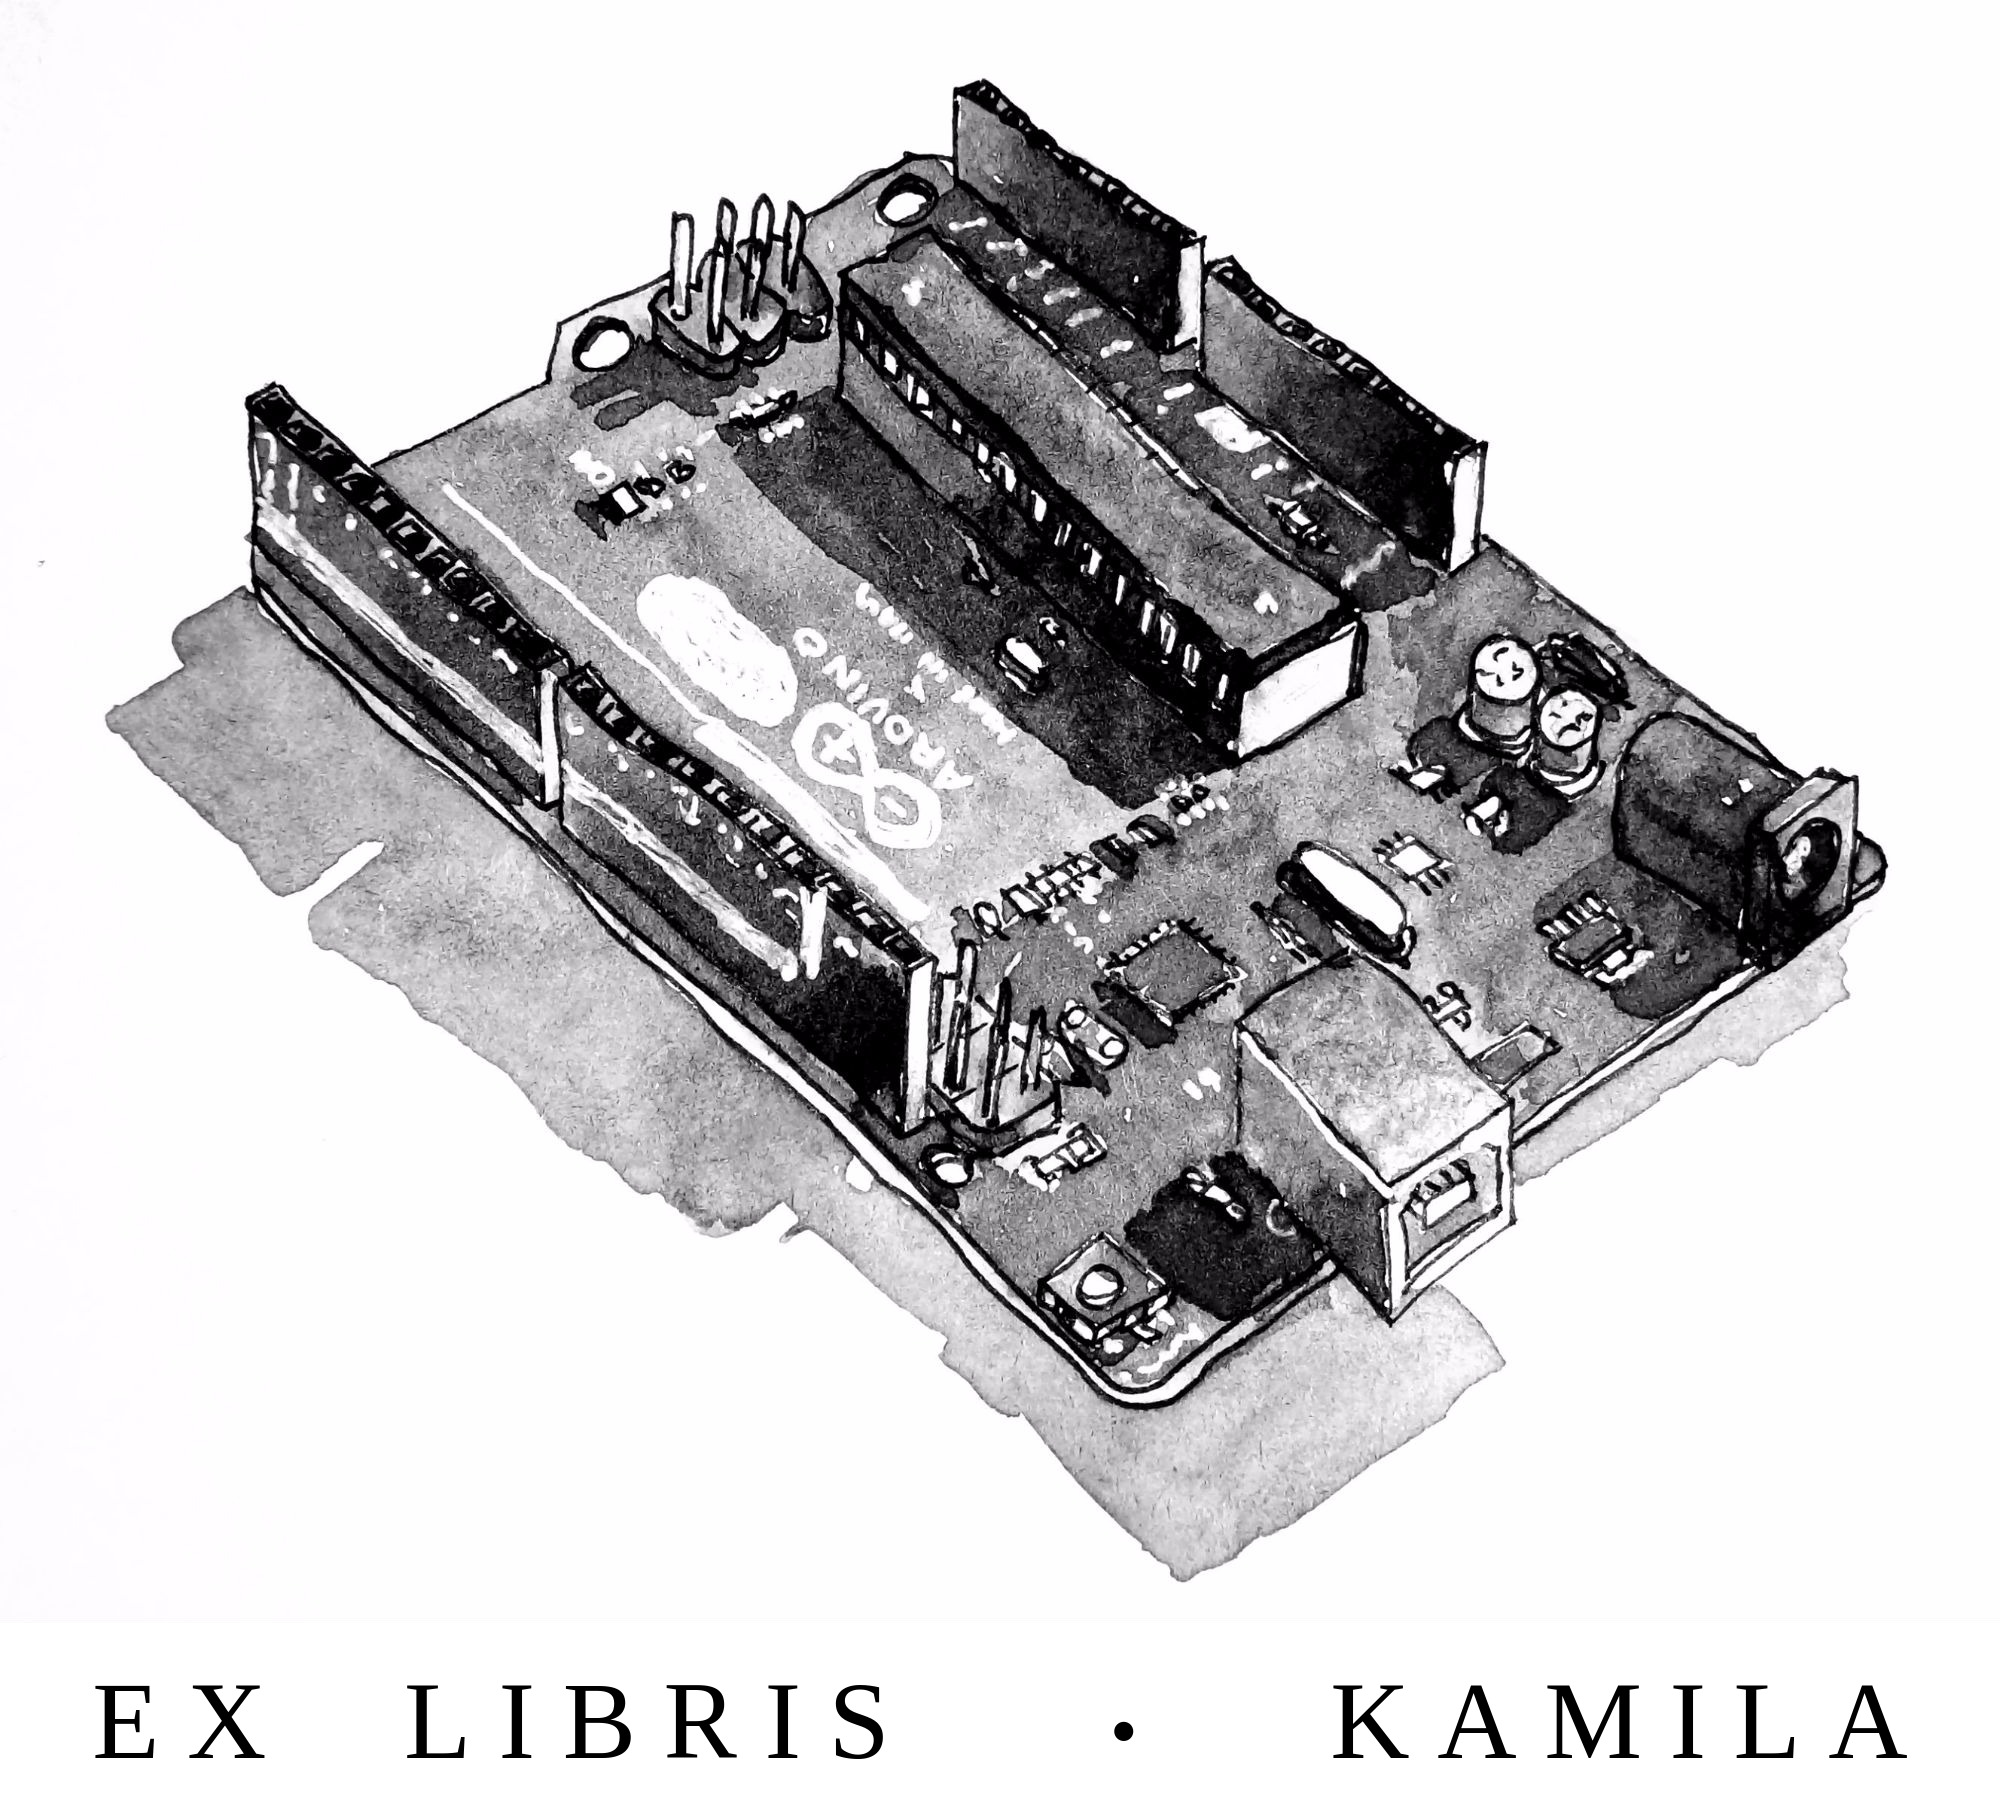
\includegraphics[width = 70mm]{arduino_dwg.jpg}

\vspace*{2cm}

Copyright \textcopyright \, Kamila Zdybał, 2017

For more documents similar to this one 

visit me on GitHub: @camillejr

To contact me personally drop me a line at:

\verb|kamilazdybal@gmail.com|

\end{center}
\newpage

% EX_LIBRIS_PAGE_TEMPLATE END ================================

\setlength{\parindent}{0cm}

\clearpage


\tableofcontents



\setlength{\parskip}{1em}
\renewcommand{\baselinestretch}{1.0}


\newpage


\section{Introduction} \label{chap:intro}








\section{Understanding substantial derivative} \label{chap:deriv}








\newpage

\begin{thebibliography}{50}



\end{thebibliography}

\end{document}
